\documentclass[10pt, aspectratio=169]{beamer}

\usetheme[progressbar=frametitle]{metropolis}
\setbeamertemplate{frame numbering}[fraction]
%\definecolor{orange}{rgb}{1,0.5,0}
%\usecolortheme[named=orange][beaver]
\usefonttheme{serif}

\useoutertheme{metropolis}
\useinnertheme{metropolis}
%\usecolortheme{beaver}
\setbeamercolor{background canvas}{bg=white}

\usepackage[italian]{babel}
\usepackage[latin1]{inputenc}
\usepackage[T1]{fontenc}
\usepackage{multicol}
\usepackage{parskip}[5pt]
\usepackage{lipsum}

\theoremstyle{definition}
\newtheorem{definizione}{Definizione}
\theoremstyle{plain}
\newtheorem{teorema}{Teorema}
\theoremstyle{example}
\newtheorem{esempio}{\itshape Esempio}
\theoremstyle{proof}
\newtheorem{dimostrazione}{\itshape Dimostrazione}
\theoremstyle{plain}
\newtheorem{soluzione}{\itshape Soluzione}

\title[Titolo in basso a destra]{Prodotti Notevoli: Esercizi}
\subtitle{Matematica per il Liceo}
\date{\today}
\author{prof. Diego Fantinelli}
\institute{Liceo Scientifico J. Da Ponte}

\begin{document}
\metroset{block=fill}

\begin{frame}
	\titlepage
\end{frame}

\begin{frame}
\frametitle{contenuti}
	\tableofcontents
\end{frame}

\section{Introduzione}

\begin{frame}[t]{Fattorizzazione "vs" Scomposizione} \vspace{10pt}
E' indispensabile partire dalla definizione di {\em polinomio}: un'espressione algebrica tra monomi non simili.\\ \vspace{10pt}
{\bfseries Scomporre} un polinomio in fattori significa esprimere - riscrivere - il polinomio come prodotto di due o pi� fattori polinomiali di grado inferiore.\\ \vspace{10pt}
La {\bfseries Fattorizzazione} � pertanto quell'operazione che permette di riscrivere un polinomio utilizzando prodotti, anzich� come una serie di somme, e i {\em fattori} sono di grado inferiore al polinomio di partenza. \\ \vspace{10pt}

\begin{teorema}
	\(16x^2 - 8x + 1 = (4x - 1)^2 = (4x - 1) \cdot (4x - 1)\)
\end{teorema}
	
\end{frame}

%\section{DERIVATE:\\ introduzione e definizioni}
%
%\begin{frame}[t]{Derivate - introduzione} \vspace{10pt}
%
%\begin{definition} \vspace{2pt}
%A prime number is a number that...
%\end{definition}
%
%\begin{esempio} \vspace{2pt}
%Lorem ipsum dolor sit amet, consectetur adipisicing elit, 
%sed do eiusmod tempor incididunt ut labore et
%dolore magna aliqua. 
%\end{esempio}
%
%\begin{dimostrazione}
%	Lorem ipsum dolor sit amet, consectetur adipisicing elit, 
%sed do eiusmod tempor incididunt ut labore et
%dolore magna aliqua.
%\[a^2+b^2=c^2\] \qed
%\end{dimostrazione} \vspace{2pt}
%
%\end{frame}

\begin{frame}[t]{Esercizio 1} \vspace{10pt}
{\Large
Sviluppare il seguente quadrato di binomio:
\((3x + 2y)^{2}\)

Sviluppando secondo la regola:
\begin{align*}
(a+b)^{2} & = a^{2}+2 a b+b^{2} \quad ponendo \quad a = 3x \quad e \quad b = 2y\\[15pt]
(3x + 2y)^{2} & = (3 x)^{2} + 2 \cdot (3x) \cdot (2y) + (2y)^{2}\\
  & = 9 x^{2}+12 x y+4 y^{2}\\
\end{align*}
}
\end{frame}

\begin{frame}[t]{Esercizio 2} \vspace{10pt}
{\Large
Sviluppare il seguente quadrato di binomio:
\((3x + 2y)^{2}\)

Sviluppando secondo la regola:
\begin{align*}
(a+b)^{2} & = a^{2}+2 a b+b^{2} \quad ponendo \quad a = 3x \quad e \quad b = 2y\\[15pt]
(3x + 2y)^{2} & = (3 x)^{2} + 2 \cdot (3x) \cdot (2y) + (2y)^{2}\\
  & = 9 x^{2}+12 x y+4 y^{2}\\
\end{align*}
}
\end{frame}

\begin{frame}[t]{Esercizio 3} \vspace{10pt}
{\Large
Sviluppare il seguente quadrato di binomio:
\((-3x - 5y)^{2}\)

Sviluppando secondo la regola:
\begin{align*}
(a+b)^{2} & = a^{2}+2 a b+b^{2} \quad ponendo \quad a = -3x \quad e \quad b = -5y\\[15pt]
(-3x - 5y^2)^{2} & = (-3x)^{2} + 2 \cdot (-3x) \cdot (-5y) + (-5y^2)^{2}\\
  & = 9x^{2} + 30xy + 25y^{2}\\
\end{align*}
}
\end{frame}

\begin{frame}[t]{Esercizio 4} \vspace{10pt}
{\Large
Sviluppare il seguente quadrato di binomio:
\((3x + 2y)^{2}\)

Sviluppando secondo la regola:
\begin{align*}
(a+b)^{2} & = a^{2}+2 a b+b^{2} \quad ponendo \quad a = 3x \quad e \quad b = 2y\\[15pt]
(3x + 2y)^{2} & = (3 x)^{2} + 2 \cdot (3x) \cdot (2y) + (2y)^{2}\\
  & = 9 x^{2}+12 x y+4 y^{2}\\
\end{align*}
}
\end{frame}

%\begin{frame}[t]{Derivate - Rappresentazione grafica} \vspace{5pt}
%Liste numerate e puntate su 2 colonne:\\ \textcolor{magenta}{$a^2+b^2=c^2$}, e capiremo come cambiare la prospettiva con cui si osserva una formula matematica\\
%\begin{multicols}{2}
%	
%\begin{enumerate}
%	\item primo elemento
%	\begin{enumerate}
%		\item uno
%		\item due
%	\end{enumerate}
%	\item secondo elemento
%	\item terzo elemento
%\end{enumerate}
%
%\begin{itemize}
%	\item primo elemento
%		\begin{itemize}
%			\item secondo elemento
%			\item terzo di tre
%		\end{itemize}
%	\item terzo elemento
%\end{itemize}
%\end{multicols}
%\end{frame}


\section{Esercitazioni}
\begin{frame}[t]{Esercizi sulle derivate} \vspace{10pt}
	\begin{soluzione}\vspace{2pt}
         Let $r, s$ be integers such that gcd$(r, s)=1$. 
         $\displaystyle \int_{0}^{\infty}x^2 - 6 x + 49 \cdot dx$ \\
         Given integers $a,b$, there exists unique 
        $x <rs$ such that 
        \begin{enumerate}
        		\item primo elemento
		\begin{itemize}
			\item secondo elemento
			\item terzo di tre
		\end{itemize}
	\item terzo elemento \qed
\end{enumerate}
	\end{soluzione}
\vspace{5pt}
        
\begin{soluzione}
Lorem ipsum dolor sit amet, consectetur adipisicing elit, 
sed do eiusmod tempor incididunt ut labore et 
dolore magna aliqua. \qed
\end{soluzione}
\end{frame}

\begin{frame}[t]{Esercizi sulle derivate} \vspace{10pt}
\begin{multicols}{2}
Hello, here is some text without a meaning.  If you read this text, you will get no information.\\ $\displaystyle \int_{0}^{\infty}x^2 - 6 x + 49 \cdot dx$, you will get no information
If you read this text, you will get no information. \\ 
%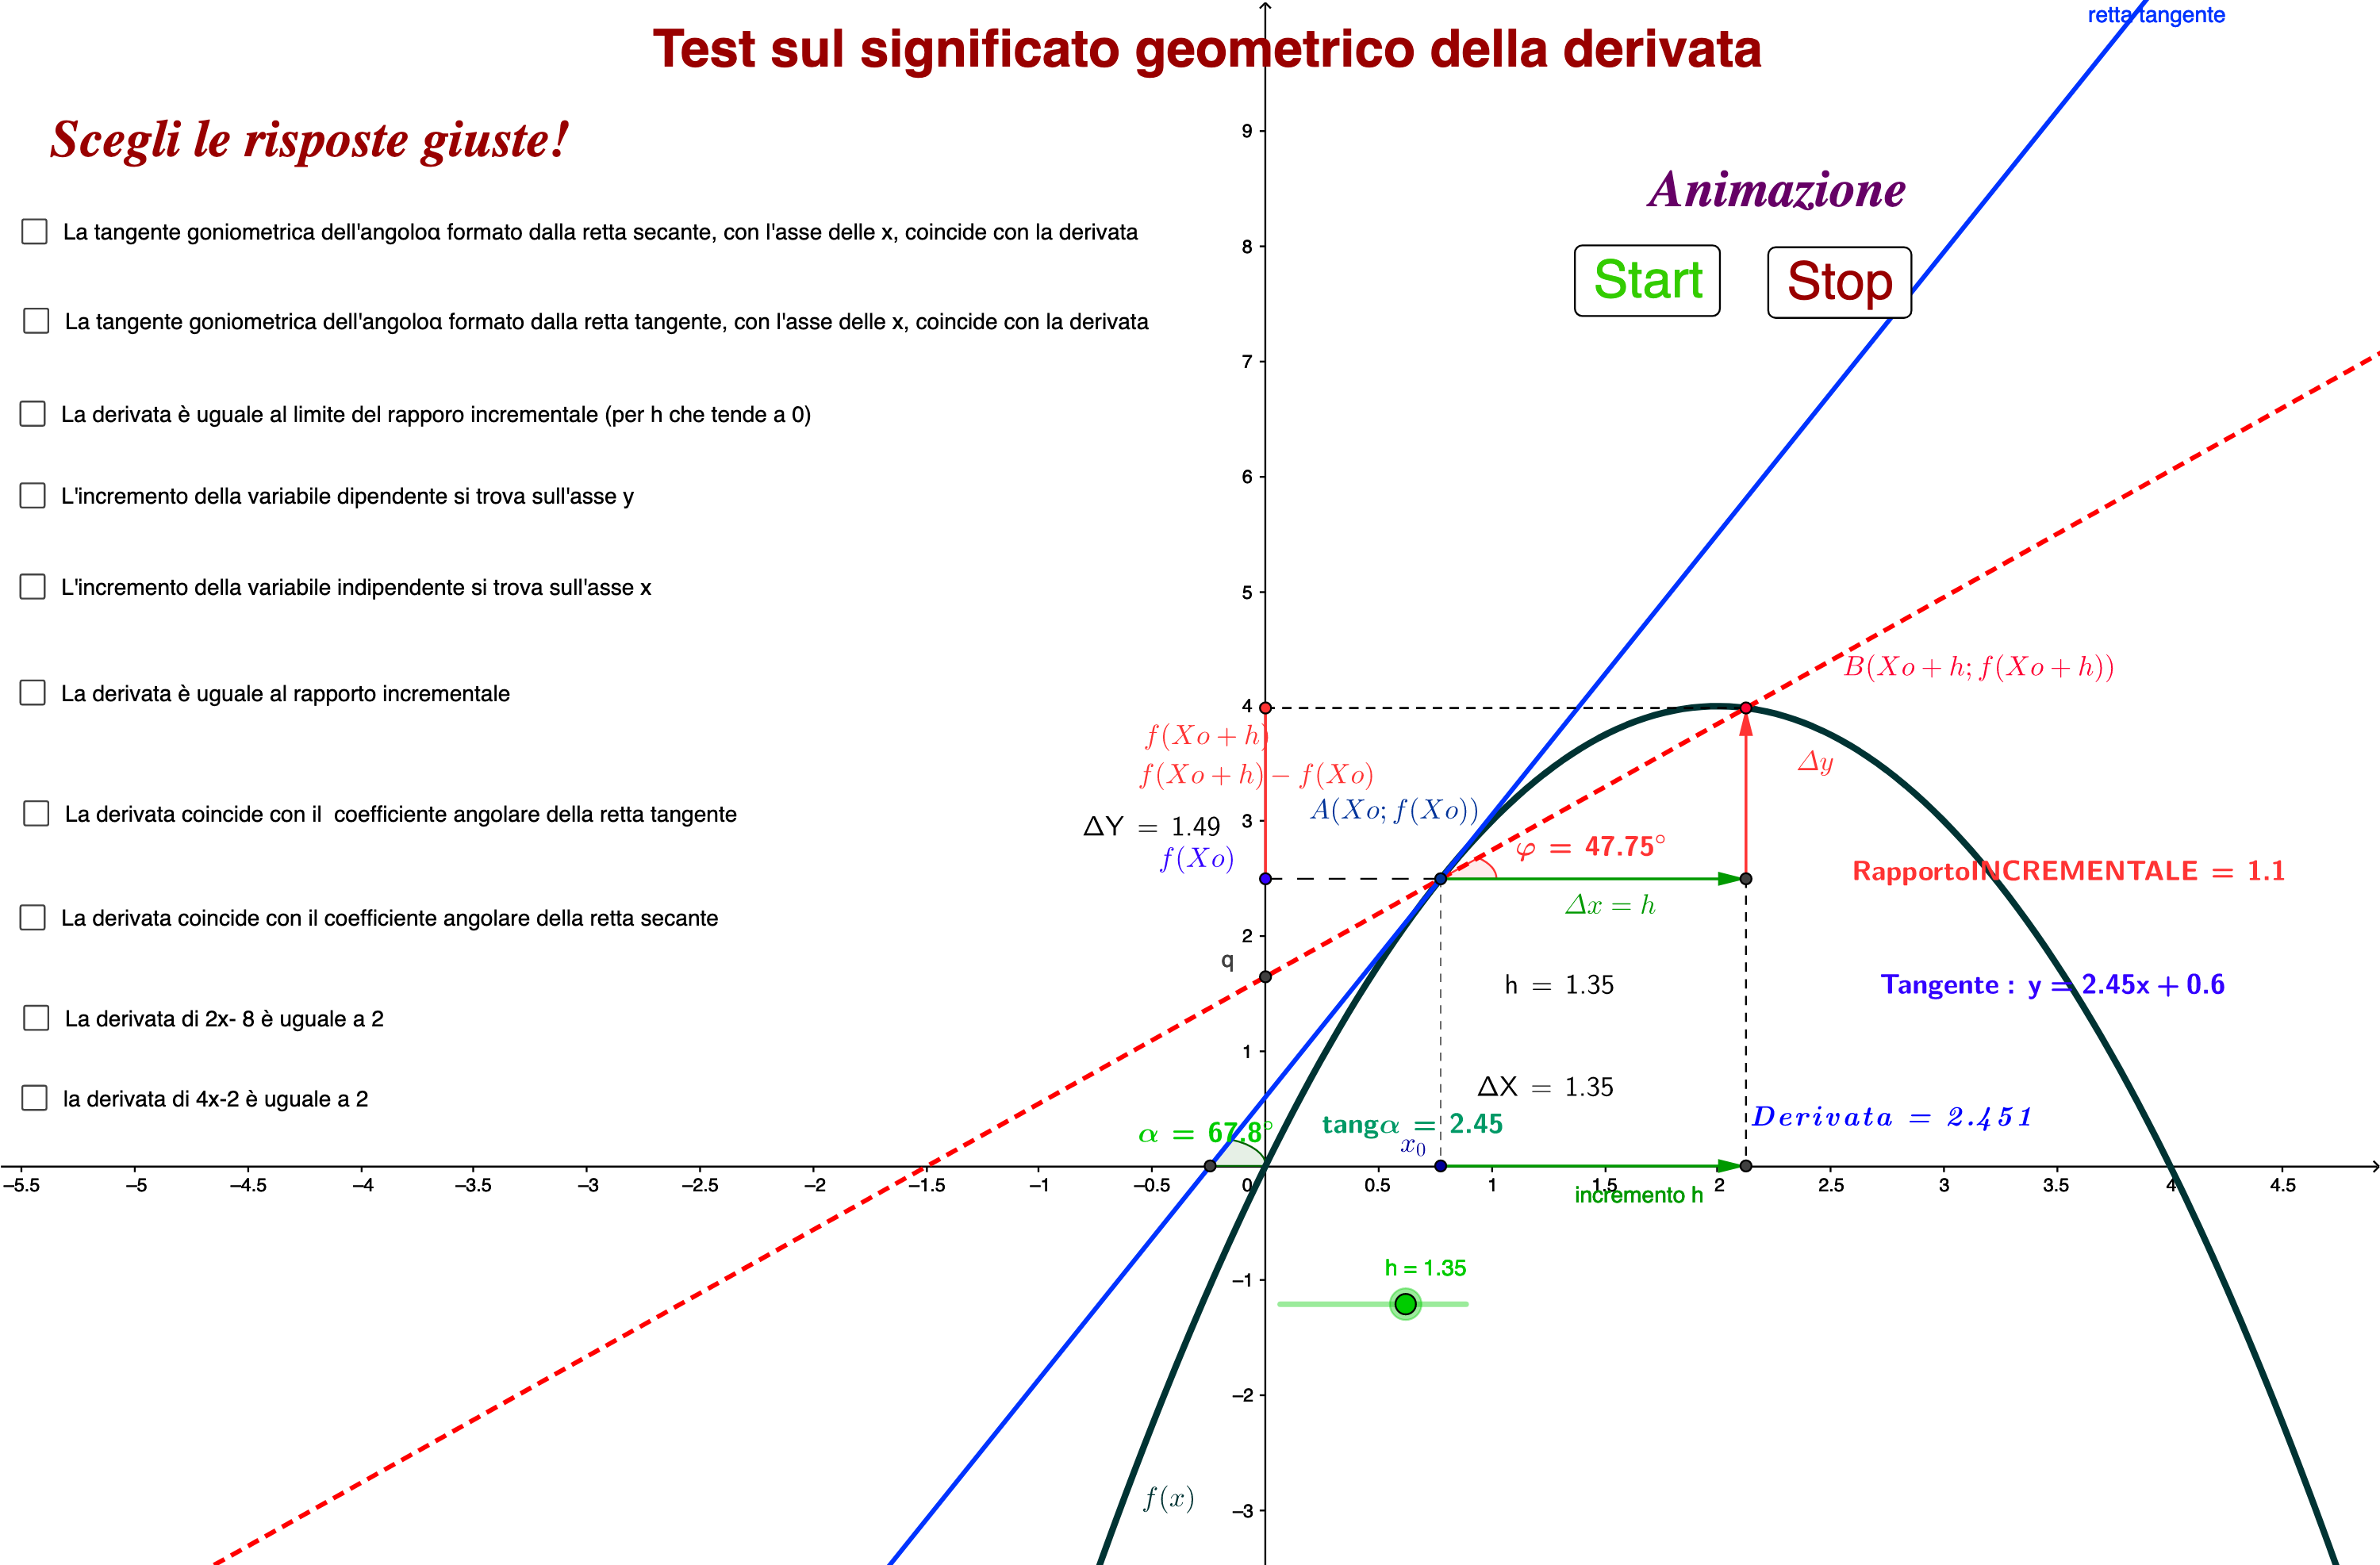
\includegraphics[scale=0.6]{derivata}\\ 
\end{multicols}
\end{frame}

\begin{frame}[t]{Esercizi sulle derivate} \vspace{10pt}
\begin{theorem}[Pythagoras] \vspace{2pt}
$ a^2 + b^2 = c^2$
\end{theorem}
\begin{corollary} \vspace{2pt}
$ x + y = y + x  $
\end{corollary}

\begin{proof} \vspace{2pt}
$\omega +\phi = \epsilon $
\end{proof}
\end{frame}

%\begin{frame}[t]{Rappresentazione Grafica delle Derivata} \vspace{10pt}
%\begin{center}
%	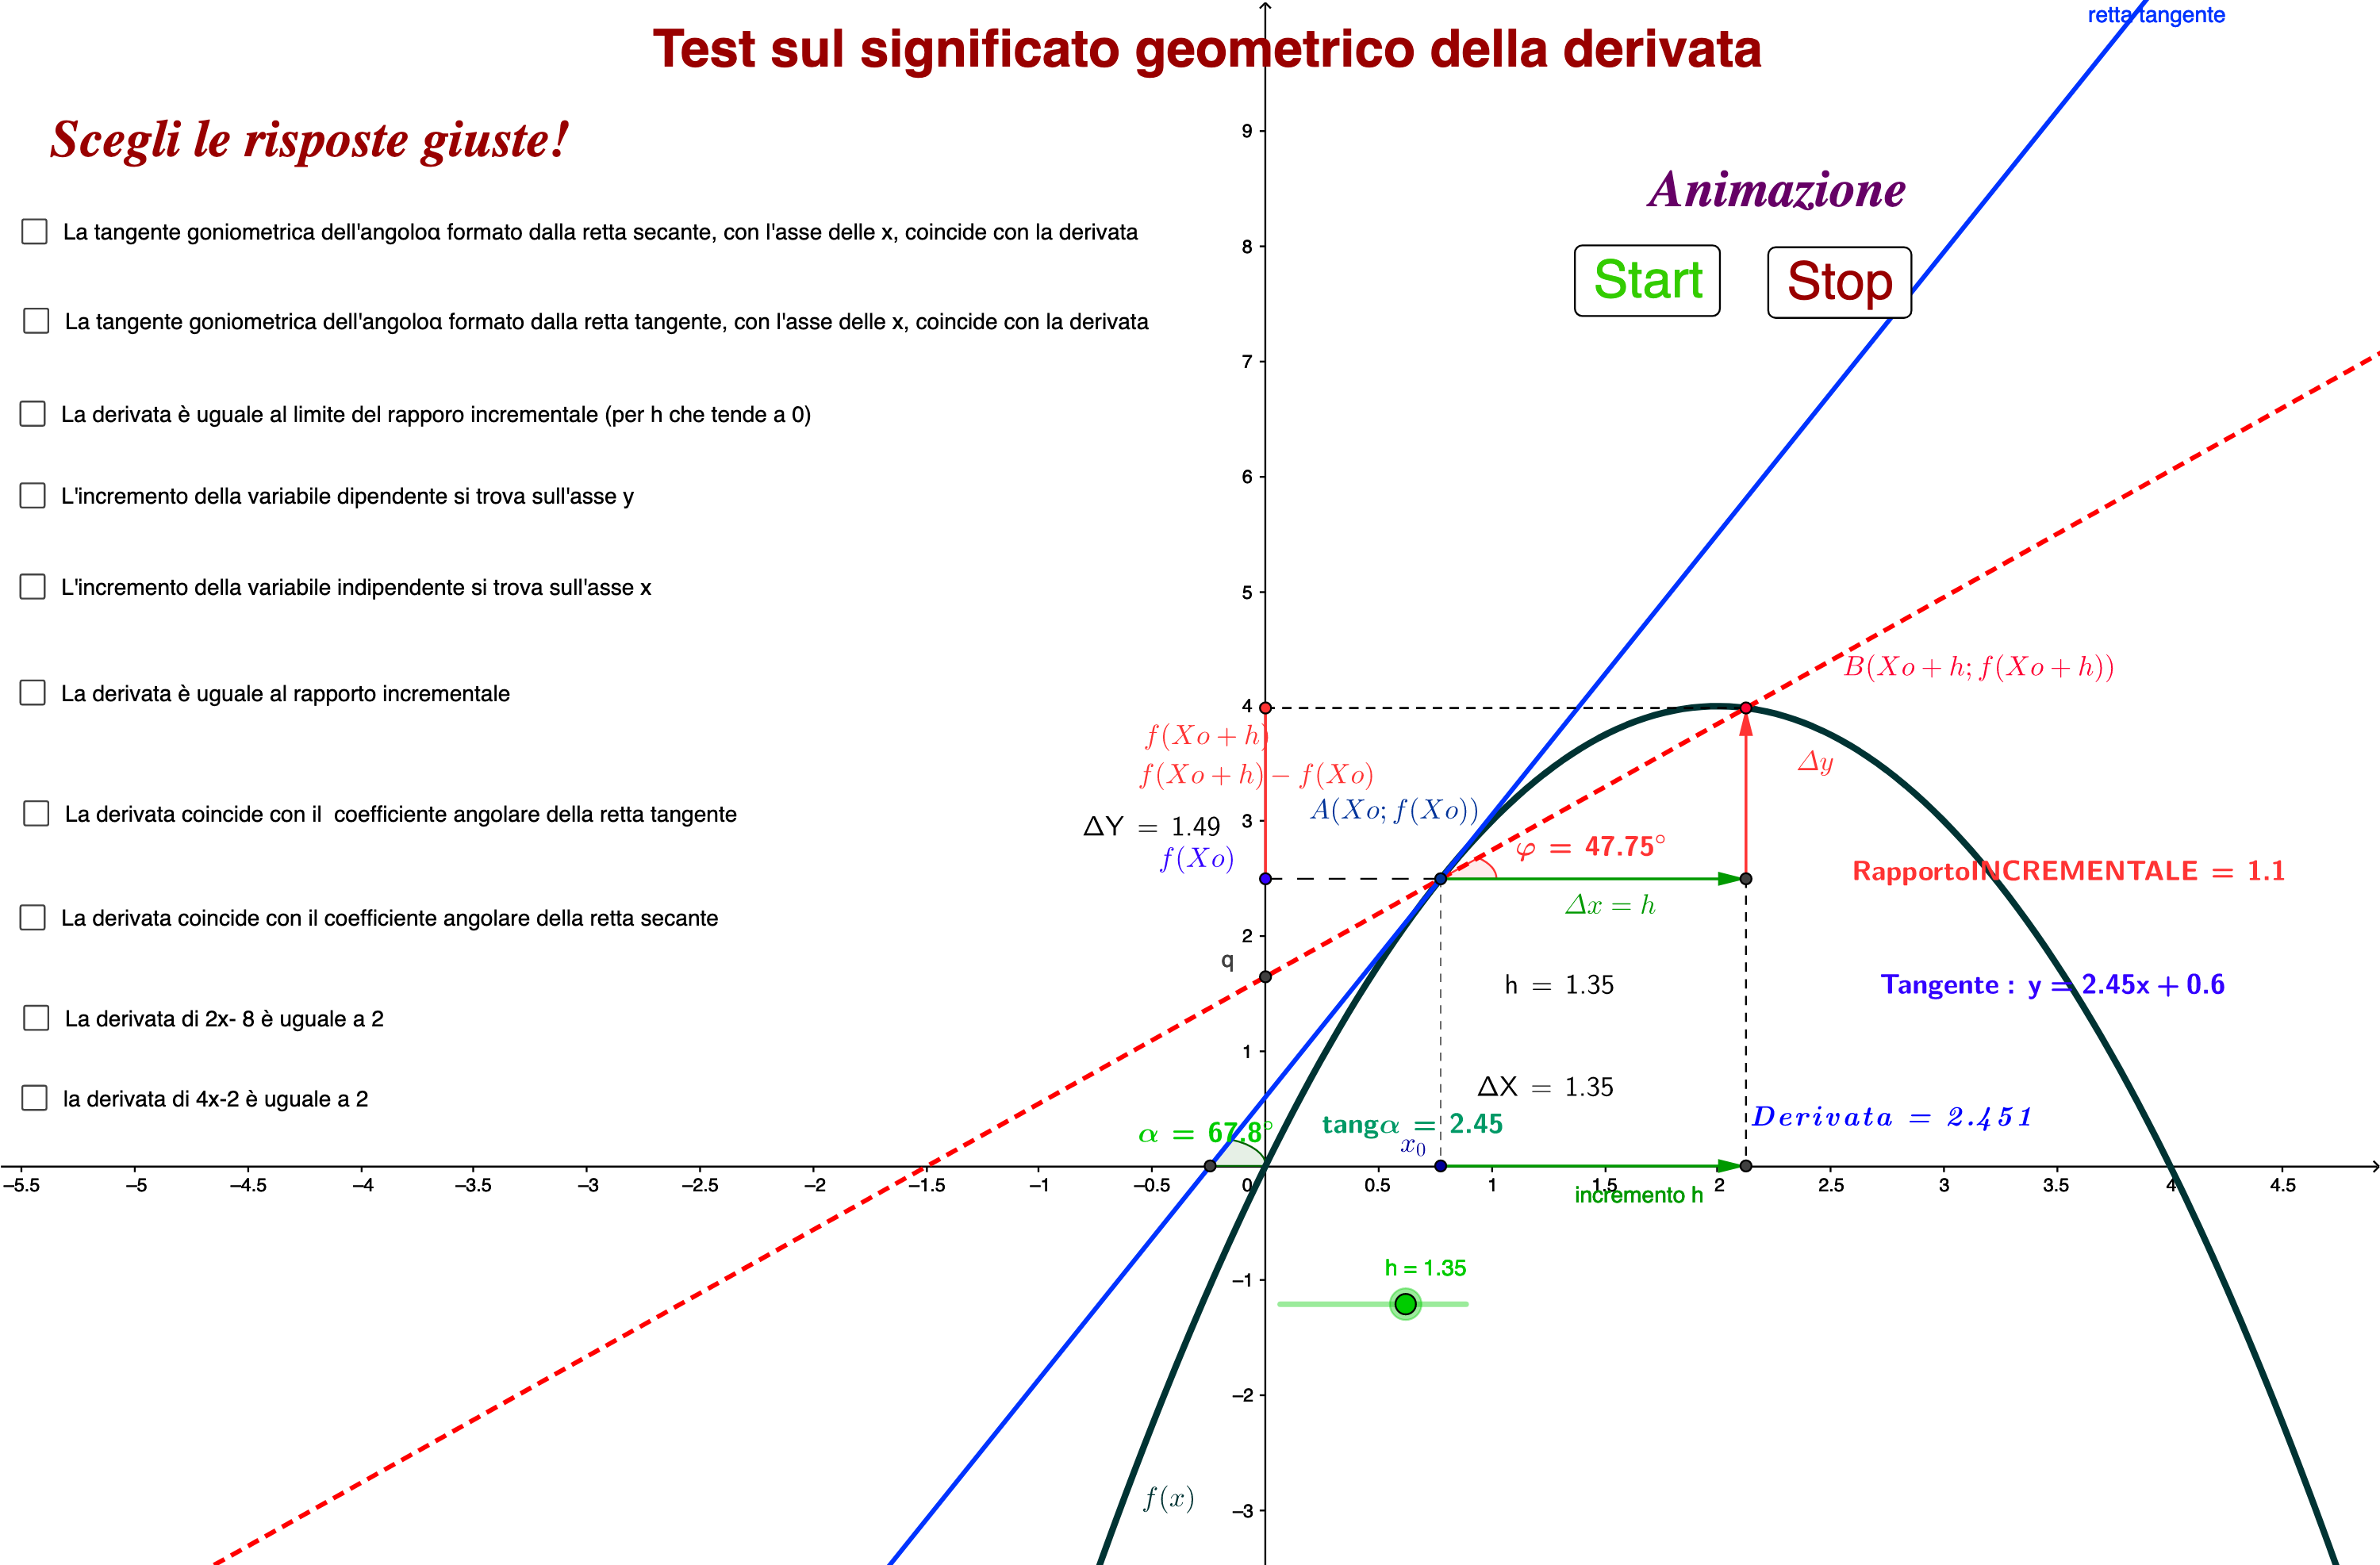
\includegraphics[scale=0.90]{derivata}
%\end{center}
%\end{frame}
\section{Compiti per casa}

\begin{frame}[label=esercizi, standout]{Esercizi sulle derivate}

         Let $r, s$ be integers such that \(gcd(r, s)=1\). \\ \vspace{10pt}
         
         $\displaystyle \int_{0}^{\infty}x^2 - 6 x + 49 \cdot dx$ \\ \vspace{10pt}
         
         
         Given integers $a,b$, there exists unique 
        $x <rs$ such that \\ \vspace{10pt}
        
        \begin{enumerate}
        		\item primo elemento
		\begin{itemize}
			\item secondo elemento
			\item terzo di tre
		\end{itemize}
	\item terzo elemento
\end{enumerate}

\vspace{5pt}
        
%\begin{soluzione}
%Lorem ipsum dolor sit amet, consectetur adipisicing elit, 
%sed do eiusmod tempor incididunt ut labore et 
%dolore magna aliqua.
%\end{soluzione}

\end{frame}
\begin{frame}[t]{Esercizi sulle derivate} 
\vspace{10pt}

\begin{alertblock}{cosa studiare} \vspace{2pt}
Lorem ipsum dolor sit amet, consectetur adipisicing elit, 
sed do eiusmod tempor incididunt ut labore et 
dolore magna aliqua.
\end{alertblock}

\pause

\begin{alertblock}{come studiare} \vspace{2pt}
Lorem ipsum dolor sit amet, consectetur adipisicing elit, 
sed do eiusmod tempor incididunt ut labore et 
dolore magna aliqua.
\end{alertblock}

\pause

\begin{alertblock}{esrcizi - revisione} \vspace{2pt}
Lorem ipsum dolor sit amet, consectetur adipisicing elit, 
sed do eiusmod tempor incididunt ut labore et 
dolore magna aliqua.
\end{alertblock}

\end{frame}

\begin{frame}[standout]{Conclusioni}
GRAZIE
\end{frame}

\end{document}